\chapter{Decision-model}
In the previous chapters are ways to identify and evaluate a situation discussed, including a case study. This means the first two steps of the OODA loop are taken, observe and orient. The next step is to decide on the right strategy. Deciding on the right strategy also includes the moment this strategy should be executed. 
This is done using a rule-based time-domain decision model. First an ontology is defined. Followed by a database of scenarios and situations as defined in the previous chapters. Combining this with the rules will result in the decision model. Thereby is the aim of this decision model to avoid communication.

\section{Decision phases}
To describe the different phases in the decision taking process. An ontology is defined to describe these phases. Thereby is shown in figure \todo{add process diagram} how these steps relate in a process diagram.
\begin{table}[H]
	\begin{tabular}{p{0.35\textwidth}|p{0.64\textwidth}}
		\toprule
		Class & Description\\
		\midrule
		Situation & The first step is to identify the encountered situation, to determine which criteria are relevant. \\
		Problem identification & The second step is to determine if there is a problem, as there is only a change in strategy needed when this is the case. \\
		Strategy & If there is a problem, a new strategy can be chosen, this is based on the evaluation of the criteria. \\
		Action & From this strategy, different actions will follow. \\
		Result & Finally the result is evaluated, in a similar manner to the problem identification. \\
		\bottomrule
	\end{tabular}
	
	\captionof{table}{Ontology used in decision model to describe phases}
	\label{tab:ontology}
\end{table}



\section{Tags for decision making}

\subsubsection{Encountered situations}
This is the first step to limit the about of steps needed to get to the right strategy. The identification process is described in table \ref{tab:situations} and section \ref{sec:situation-identification}.
\begin{table}[H]
	\begin{tabular}{p{0.35\textwidth}|p{0.64\textwidth}}
		\toprule
		Tag & Description\\
		\midrule
		Passing & The paths of both ships are in opposite direction, and do not cross. \\
		Crossing & The final direction of both ships differs, but they do cross. \\
		Merge & The final direction of both ships is the same. \\
		Over-taking & The paths of both ships are the same but at different speeds. \\
		\bottomrule
	\end{tabular}
	
	\captionof{table}{Tags for different situations}
	\label{tab:situations}
\end{table}

\subsubsection{Identification of problem}
To identify if there is a problem, different criteria are being evaluated. These criteria are described in chapter \ref{ch:criteria}. In table \ref{tab:identification-criteria} the nodes and branch tags within the decision tree are discussed to evaluate if there is a problem, and what kind of problem there is. 
\begin{table}[H]
	\begin{tabular}{p{0.35\textwidth}|p{0.64\textwidth}}
		\toprule
		Tag & Evaluation \\
		\midrule
		\acf{CPA} & Good; Too close \\
		Crossing point & In front; Behind \\
		Crossing distance & Good; Too close \\
		Relative speed & Faster; Same speed; slower \\
		\bottomrule
	\end{tabular}
	
	\captionof{table}{Tags used for identification of a problem}
	\label{tab:identification-criteria}
\end{table}

\subsubsection{Possible strategies}
\begin{table}[H]
	\begin{tabular}{p{0.35\textwidth}|p{0.64\textwidth}}
		\toprule
		Tag & Description\\
		\midrule
		Follow planned path & \\
		Move away from other path & \\
		Stay parallel for longer & \\
		Adjust speed & \\
		Abort over-taking & \\
		Move away from other position & Check if this is to starboard, otherwise communicate \\
		Communicate & \\
		\bottomrule
	\end{tabular}
	
	\captionof{table}{Tags for different strategies}
	\label{tab:strategies}
\end{table}

\subsubsection{Possible actions}
To execute a strategy, different actions are taken. These action are a combination of an action type, and a moment to execute action. In table \ref{tab:actions} and \ref{tab:time-domain-action} these are described.
\begin{table}[H]
	\begin{tabular}{p{0.35\textwidth}|p{0.64\textwidth}}
		\toprule
		Tag & Description\\
		\midrule
		Continue without change & \\
		Starboard & \\
		Portside & \\
		Slow down & \\
		Speed-up & \\
		\bottomrule
	\end{tabular}
	
	\captionof{table}{Types of actions}
	\label{tab:actions}
\end{table}

\begin{table}[H]
	\begin{tabular}{p{0.35\textwidth}|p{0.64\textwidth}}
		\toprule
		Tag & Description\\
		\midrule
		Now & \\
		In ... minutes & \\
		After action ... & \\
		\bottomrule
	\end{tabular}
	
	\captionof{table}{Time-domain for action}
	\label{tab:time-domain-action}
\end{table}

\subsubsection{Result}
\begin{table}[H]
	\begin{tabular}{p{0.35\textwidth}|p{0.64\textwidth}}
		\toprule
		Tag & Description\\
		\midrule
		CPA & \\
		Perceived risk & \\
		\bottomrule
	\end{tabular}
	
	\captionof{table}{Tags for safe situation criteria}
	\label{tab:criteria-safe-situation}
\end{table}

\begin{table}[H]
	\begin{tabular}{p{0.35\textwidth}|p{0.64\textwidth}}
		\toprule
		Tag & Description\\
		\midrule
		Safe situation & \\
		Communicate & \\
		\bottomrule
	\end{tabular}
	
	\captionof{table}{Tags for results}
	\label{tab:result}
\end{table}


\section{Decision trees}
Static analysis to identify the problem can be found in figure \ref{fig:Crossing_decision_tree}-\ref{fig:Passing_decision_tree}.

\begin{figure}[p]
	\centering
	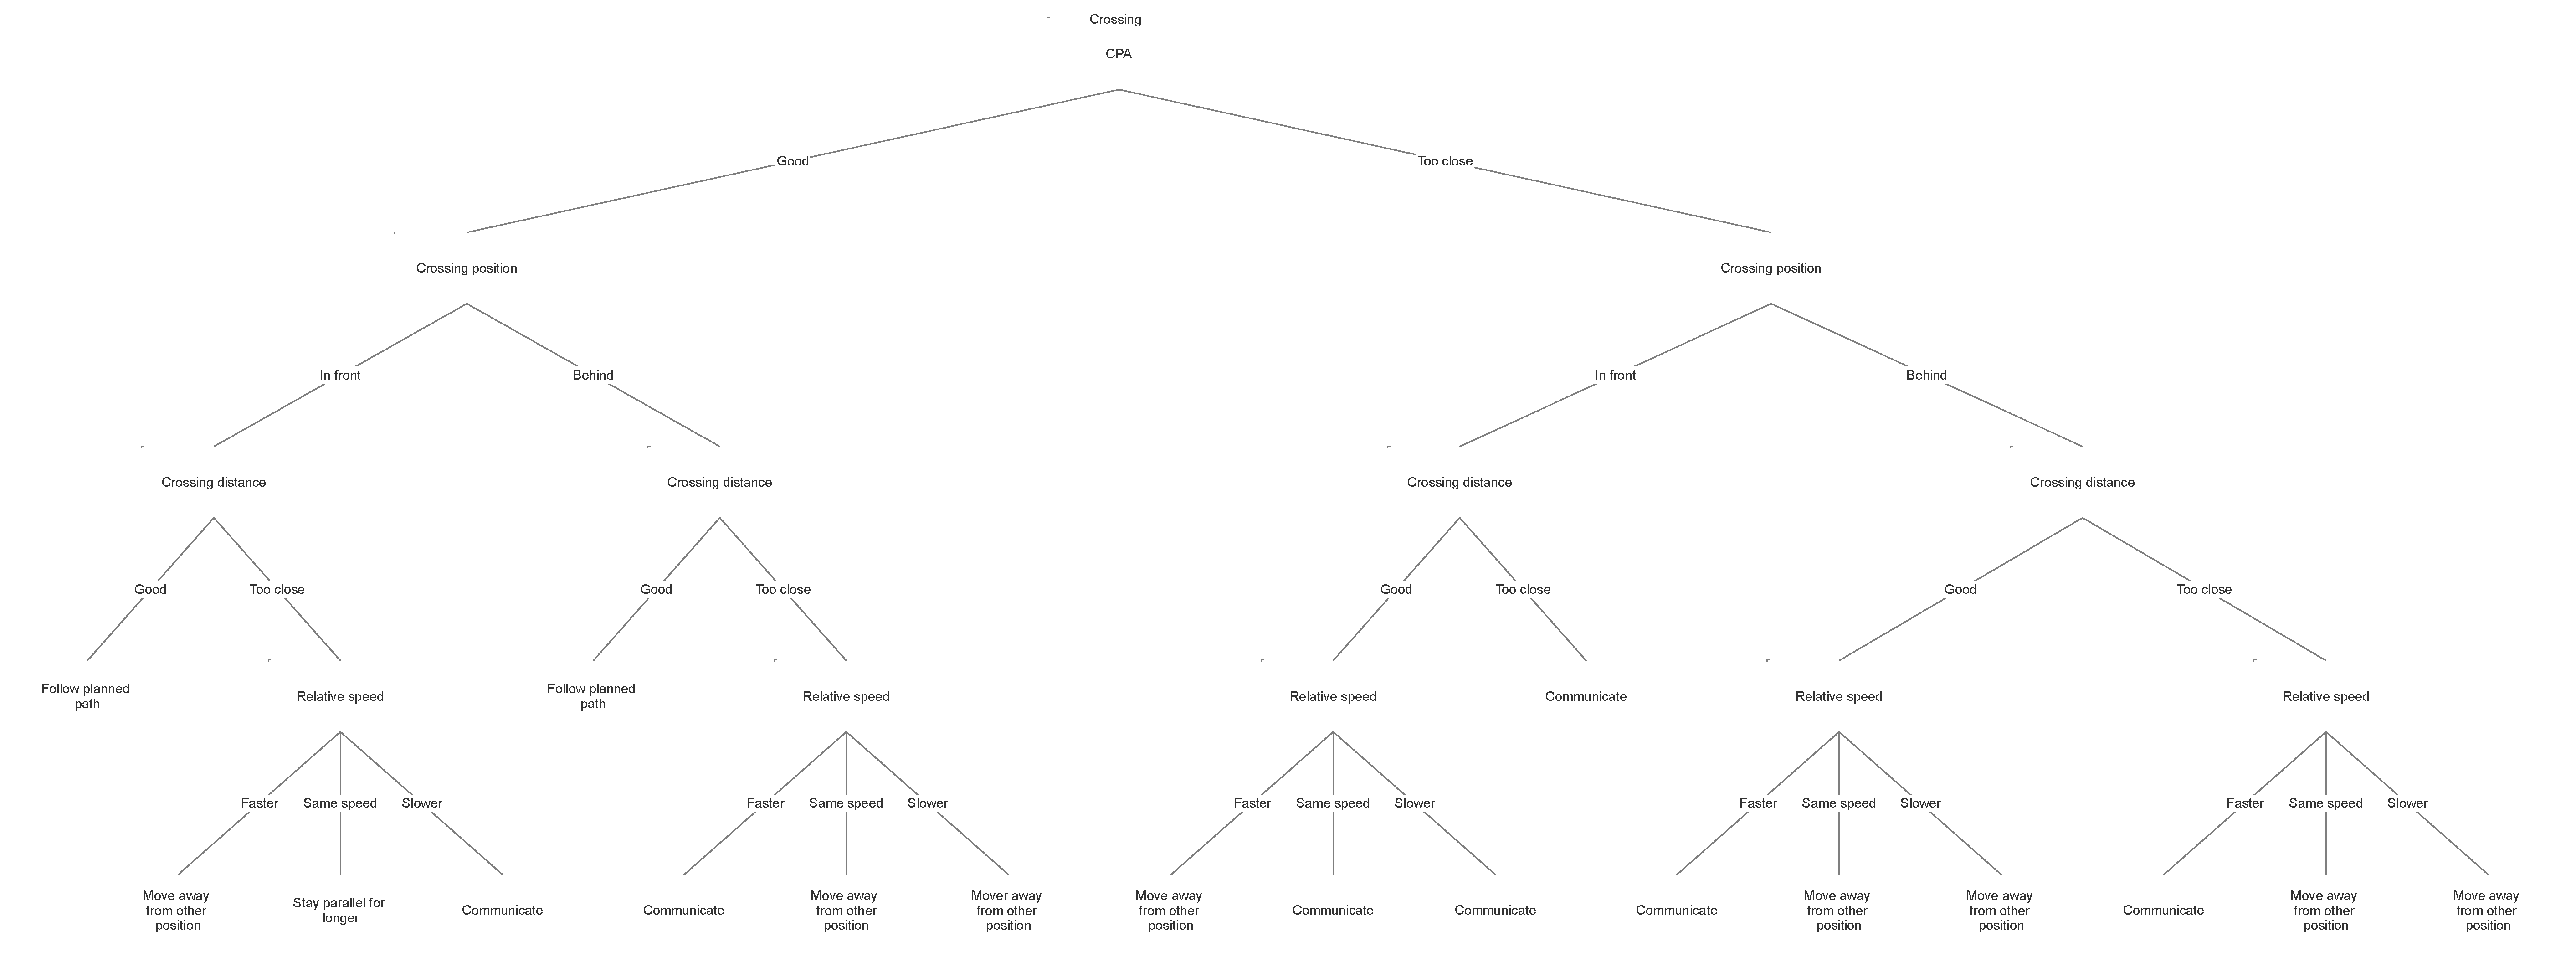
\includegraphics[width=.9\textheight, angle =90 ]{Crossing_decision_tree.png}
	\caption{Decision tree when crossing}
	\label{fig:Crossing_decision_tree}
\end{figure}


\begin{figure}[p]
	\centering
	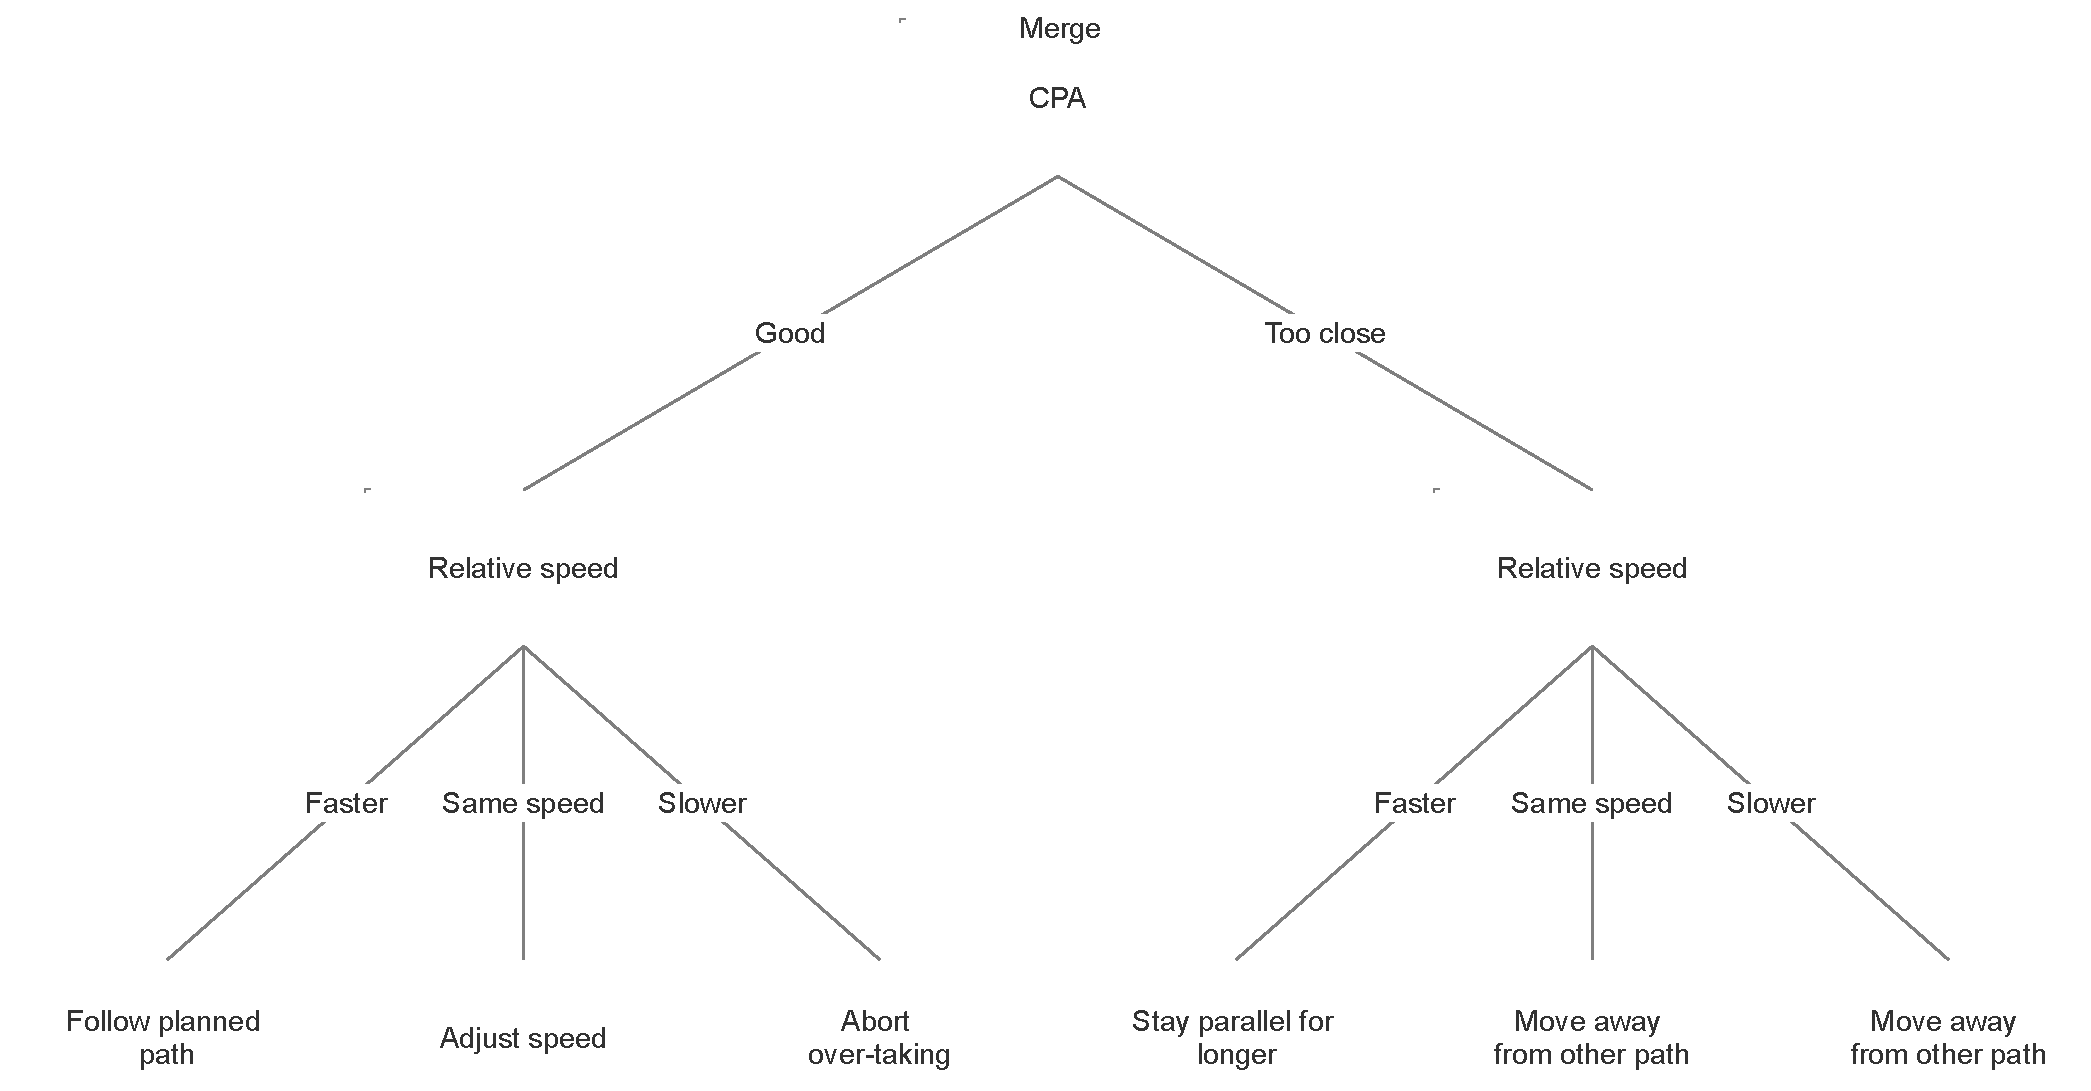
\includegraphics[width=.95\textwidth]{Merge_decision_tree.png}
	\caption{Decision tree when merging}
	\label{fig:Merge_decision_tree}
\end{figure}


\begin{figure}[p]
	\centering
	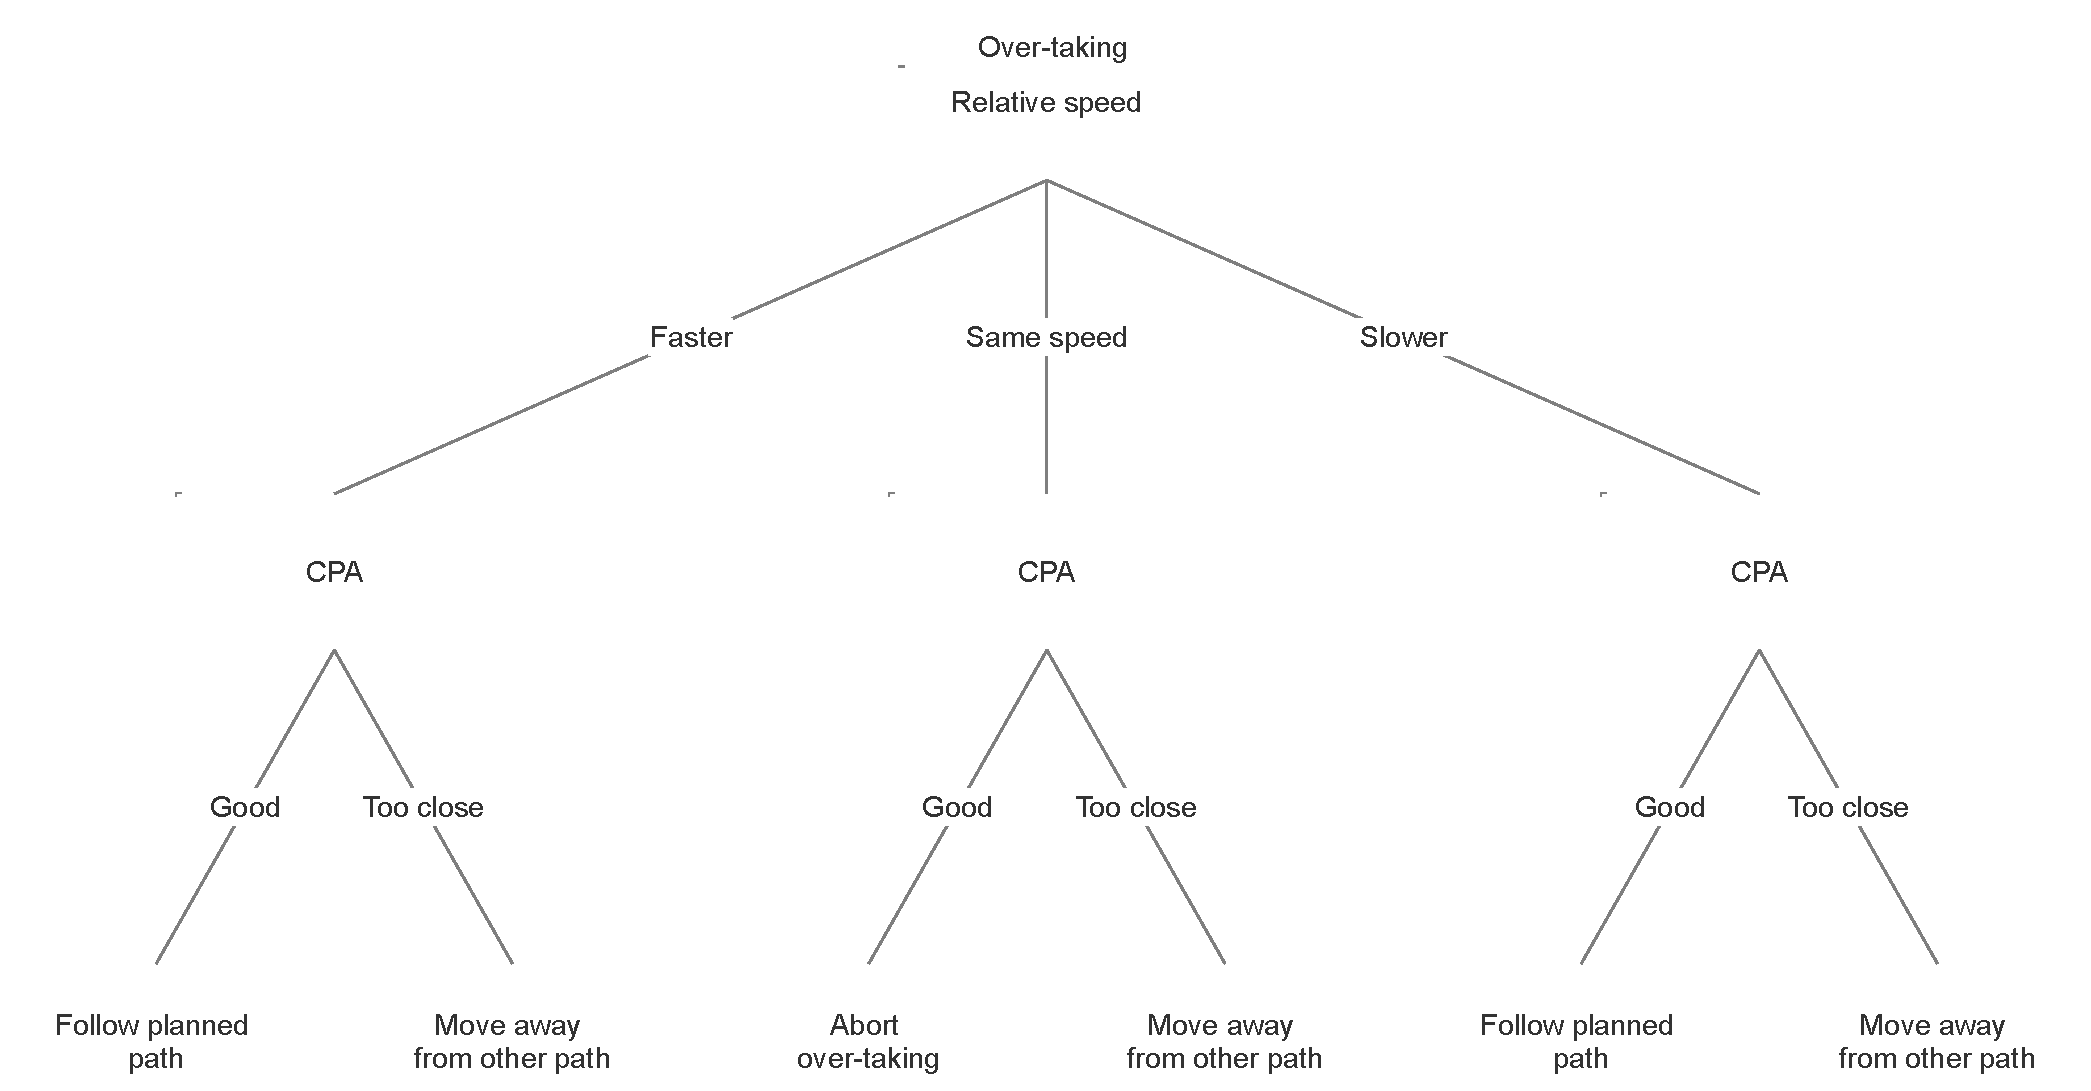
\includegraphics[width=.9\textwidth]{Over-taking_decision_tree.png}
	\caption{Decision tree when over-taking}
	\label{fig:Over-taking_decision_tree}
\end{figure}


\begin{figure}[p]
	\centering
	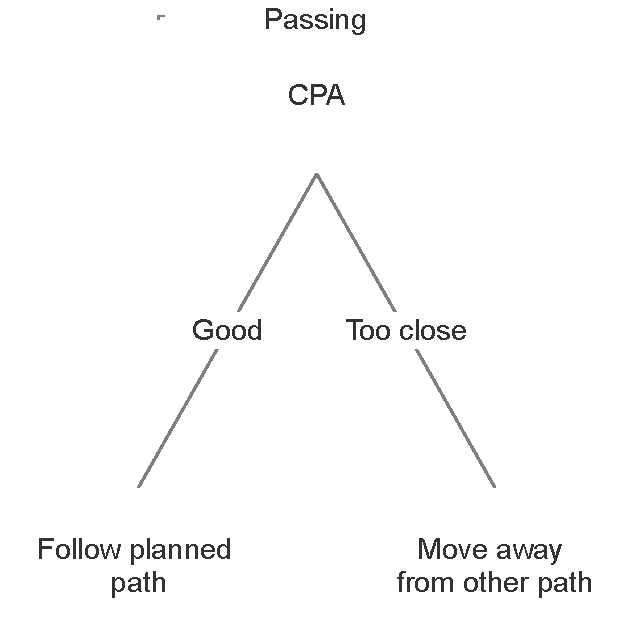
\includegraphics[width=0.2\textwidth]{Passing_decision_tree.png}
	\caption{Decision tree when passing}
	\label{fig:Passing_decision_tree}
\end{figure}


